\newpage
\section{Auswertung}
\subsection{Analyse der Stabilität}
Durch die Darstellung der Stabilitätsbedingung aus Gleichung \ref{eq:stabil} der jeweiligen Spiegelkonfiguration
lässt sich durch die Messungen aus Tabelle \ref{tab:stabil} die folgenden Aussagen treffen.

Für die beiden Speigelkonfigurationen konkav/konkav (mit $r_1=r_2=1400\,$mm) und plan/konkav ($r_1=\infty {,} r_2=1400\,$mm)
lässt sich das Stablitätsprodukt $g_1g_2$ gegen die Resonatorlänge $L$ auftragen.
Extrapoliert man die Messwerte mithilfe der geeigneten Funktion die aus Gleichung \ref{eq:stabil} hervorgeht (Linear- und Quadratfunktion)
so ergibt sich für die konkav/konkav Konfiguration die theoretische maximale Resonatorlänge von $L_{\text{max}}=2,80\,$m (in Abbildung \ref{fig:stabil} in rot dargestellt), 
sowie eine kritische Stabilität bei $L_{\text{kri}}=1,40\,$m.

\begin{figure}[H]
    \center
    \includegraphics[width=0.8\textwidth]{plots/stabilitätsbedingung.pdf}
    \caption{Das Stabilitätsprodukt $g_1g_2$ der beiden Spiegelkonfigurationen (konkav/konkav in blau und plan/konkav in gelb) mit der jewiligen Extrapolation (gestrichelt blau/gelb).
    Die kritischen Stabilitäten sind durch die rot geschrichelten Linin hervorgehoben.}
    \label{fig:stabil}
\end{figure}
\label{sec:Auswertung}

Die jeweilige gemessene Leistung $P$ bei betrachteter Resonatorlänge $L$ ist der Tabelle \ref{tab:stabil} und 
der Abbildung \ref{fig:leistung} zu entnehmen. Es wird deutlich, dass die Konfiguration der konkav/konkav Spiegeln keine Resonatorlänge $L$ gefunden 
werden kann für diese der Laserbetreib nicht aufrecht gehalten werden kann. Eine Aussage über die plan/konkave Konfiguration 
lässt sich aufgrund der Daten nicht treffen.
\begin{figure}[H]
    \center
    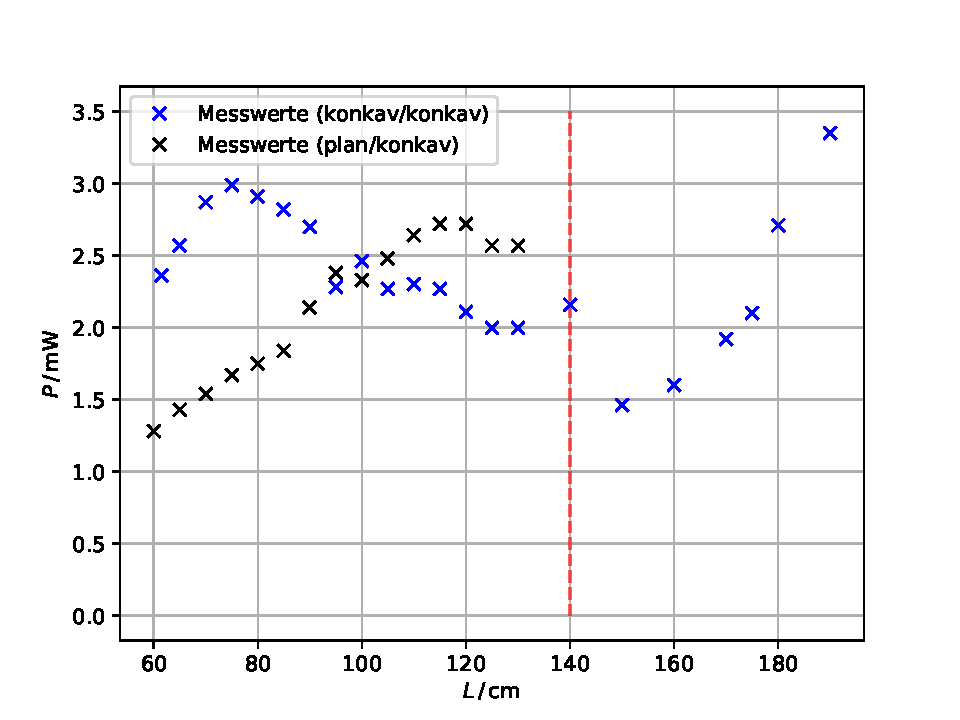
\includegraphics[width=0.7\textwidth]{plots/leistung.pdf}
    \caption{Die gemessene Leistung $P$ in Abhängigkeit der Resonatorlänge $L$ für die beiden Speigelkonfigurationen.}
    \label{fig:leistung}
\end{figure}

\subsection{Analyse der TEM-Moden}
\subsubsection{TEM$_{00}$-Moden}
Die Leistung $P$ des Laserlichtes in Abhängigkeit von der x-Position der auf dem Schirm sichtbaren Mode lässt sich mit
einer Photodiode vermessen. Dies lässt sich mithilfe einer Zersteuungslinse vergrößern und erleichtert so die Messung.
Für die Grundmode TEM$_{00}$ ergibt sich nach
\begin{equation}
    I_{m0}(x)\sim H_m \left(\frac{x}{w}\right)^2\exp\left(-2\left(\frac{x}{w}\right)^2\right)
\end{equation}
mit der Hermiteschen Polynom $H_m$, die Intensitätsverteilung $I_{00}$ für die TEM$_{00}$-Mode von
\begin{equation}
    I_{00}\sim \exp\left(-2\left(\frac{x}{w}\right)^2\right)
\end{equation}

Die Leistungen in Abhängigkeit der x-Position lässt sich aus der Tabelle \ref{tab:TEM00} entnehmen.
In Abbildung \ref{fig:TEM00} sind diese Messwerte graphisch dargestellt. Darüber hinaus werden die Messwerte durch 
die Theoriefunktion interpoliert, welche die Form
\begin{equation}
    I(x)=I_0\cdot \exp\left(-2\frac{(x-x_0)^2}{w^2}\right)
\end{equation}
aufweist.
Es ergeben sich für die Parameter die Werte
\begin{align*}
    I_0&=0,031\,\text{mW}{,}\\
    x_0&=-0,32\,\text{mm}{,}\\
    w&=6,71\,\text{mm}.
\end{align*}
\begin{figure}
    \center
    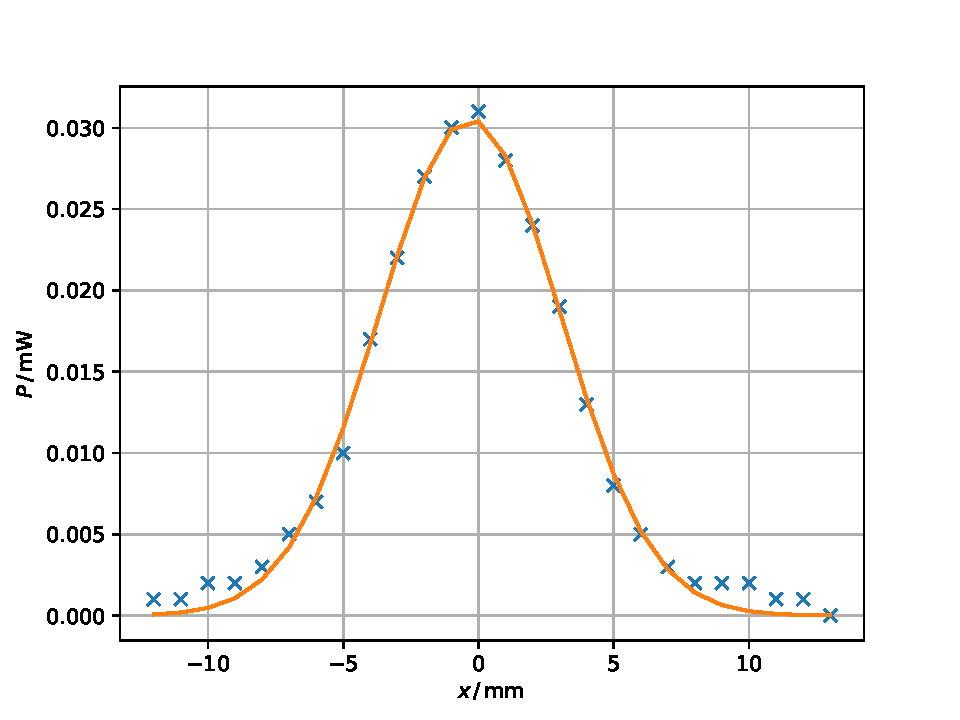
\includegraphics[width=0.8\textwidth]{plots/TEM00.pdf}
    \caption{Die gemessene Leistung $P$ der TEM$_{00}$-Mode in Abhängigkeit der x-Position.}
    \label{fig:TEM00}
\end{figure}


\subsubsection{TEM$_{10}$-Moden}
Für die TEM$_{10}$-Mode folgt demnach ein $m=1$, daher ergibt sich die theoretische Intensitätsverteilung
zu 
\begin{equation}
    I(x)=I_0\cdot 4\left(\frac{(x-x_0)^2}{w^2}\right)\cdot\exp\left(-2\frac{(x-x_0)^2}{w^2}\right).
\end{equation}
Die Interpolation liefert die Werte
\begin{align*}
    I_0&=3,33\,\text{mW}{,}\\
    x_0&=0,60\,\text{mm}{,}\\
    w&=7,76\,\text{mm}.
\end{align*}
Die Leistungen $P$ zu den zugehörigen x-Positione liefern die Abbildung \ref{fig:TEM10} resultierend aus den Messwerten aus Tabelle \ref{tab:TEM10}.
\begin{figure}
    \center
    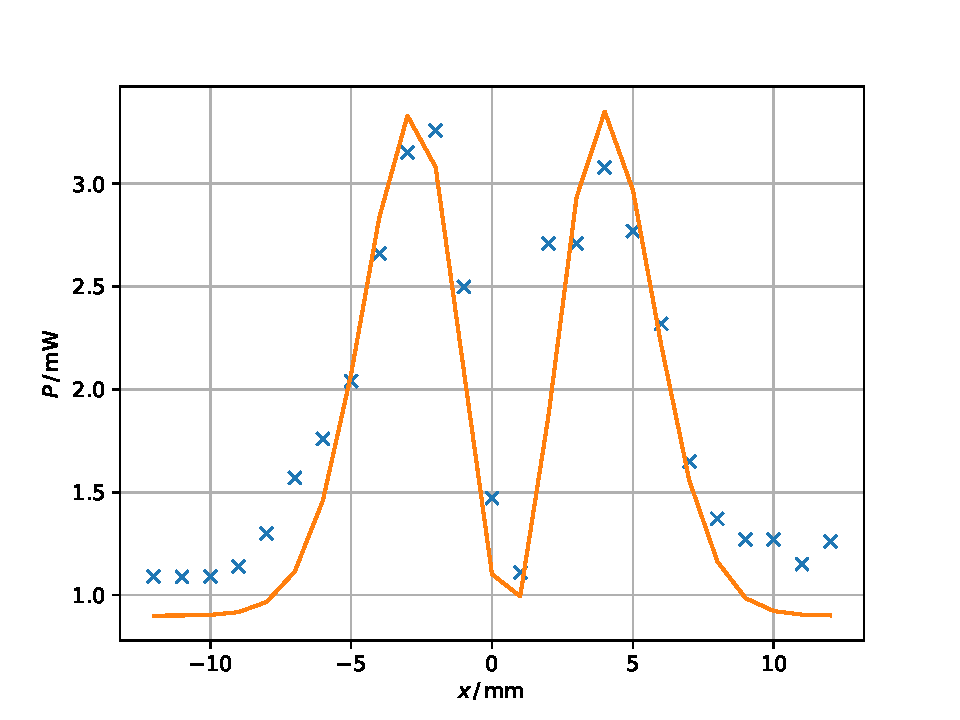
\includegraphics[width=\textwidth]{plots/TEM10.pdf}
    \caption{Die gemessene Leistung $P$ der TEM$_{10}$-Mode in Abhängigkeit der x-Position.}
    \label{fig:TEM10}
\end{figure}



\subsection{Analyse der Polarisation}
Die gemessene Leistung $P$ in Abhängigkeit der Winkelstellung $\theta$ des Linearpolarisators ist in Tabelle \ref{tab:pol} zu finden.
Die Abhängigkeit der Intensität zum Winkel $\theta$ ergibt sich nach
\begin{equation}
    I=I_0\cos^2(\theta+\theta_0).
\end{equation}
Aus der Interpolation ergeben sich folgende Werte für die Parameter
\begin{align*}
    I_0&=1,84\,\text{mW}{,}\\
    \theta_0&=1,387\,\text{rad}{,}=79,5°.
\end{align*}
In Abbildung \ref{fig:pol} sind die Messdaten aus Tabelle \ref{tab:pol} sowie die Interpolation grafisch dargestellt.
\begin{figure}
    \center
    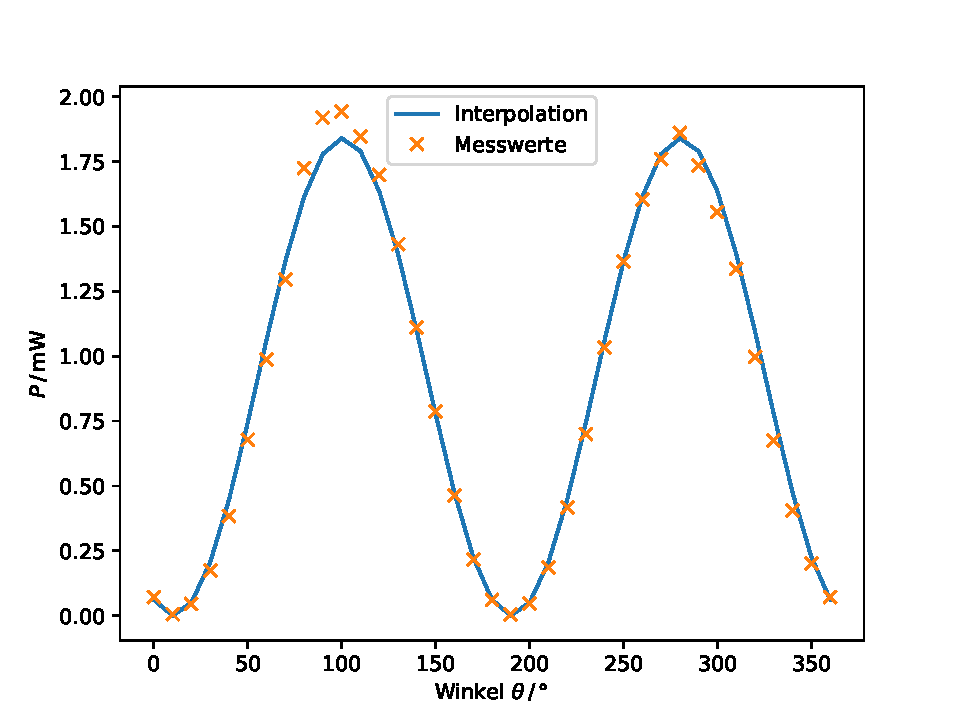
\includegraphics[width=\textwidth]{plots/pol.pdf}
    \caption{Die Leistung $P$ in Abhängigkeit des Polarisationswinkels $\theta$.}
    \label{fig:pol}
\end{figure}


\subsection{Analyse der Wellenlänge}
Mit Hilfe der Beugung an einem Gitter mit der Gitterkonstante $d$ können die Abstände $A_n$
der n-ten Interferenzmaxima zum Hauptmaximum $n=0$ vermessen werden. Dabei ist das Beugungsgitter
in einem Abstand $L$ zum Schirm positioniert.\\

Aus der Bedingung für eine konstruktive Interferenz nach
\begin{equation}
    \Delta g = n \cdot \lambda
\end{equation}
mit einem Gangunterschied von
\begin{equation}
    \Delta g = d \cdot \sin(\beta_n)
\end{equation}
und dem Beugungswinkel
\begin{equation}
    \beta_n=\arctan(A_n/L)
\end{equation}
ergibt sich für das n-te Maximum die Wellenlaänge $\lambda$ aus
\begin{equation}
    \lambda=\frac{d\cdot \sin(\arctan(A_n/L))}{n}=\frac{d\cdot A_n}{n\sqrt{A_n^2+L^2}}
\end{equation}
welche gemäß der gaußschen Fehlerfortpflanzung mit der Unsicherheit $\sigma(\lambda)$ behaftet ist.
Für die Fehler für die Abmessung zwischen Gitter und Schirm, seien im folgenden
\begin{equation*}
    \sigma(A_n)=\sigma(L)=5\,\text{mm}
\end{equation*}
angenommen.

\begin{table}
    \centering
    \caption{Die Berechneten Wellenlängen $\lambda$ zu den jeweiligen Vermessenden $n$-ten Beugungsmaxima der jeweiligen Gittern mit 
    den Gitterkonstanten $d$ aus dem Abstand $A_n$ zum Hauptmaxima bei einer Entfernung $L$ zum Schirm.}
    \begin{tabular}{c c c c c}
        \toprule
        Gitterkonstante $d\,/\,$mm & Ordnung $n$ & Abstand $A_n\,/\,$mm & Abstand $L\,/\,$mm & Wellenlänge $\lambda\,/\,$nm\\
        \midrule
        1/1200  &   1   &   371   &   312,5   &   637,35\\
        1/600   &   1   &   130   &   312,5   &   642,25\\
        1/600   &   2   &   379   &   312,5   &   642,95\\
        1/100   &   1   &   20      &   312,5   &   638.69\\
        1/80    &   1   &   17,5    &   312,5   &   698,90\\
        1/80    &   2   &   50      &   312,5   &   658,29\\
        1/80    &   3   &   101     &   312,5   &   643,57\\   
        \bottomrule
    \end{tabular}
    \label{tab:wellen}
\end{table}
Daraus folgt ein Mittelwert für die Wellenlänge von $\bar{\lambda}=651,71\,\text{nm}$.
